\documentclass[letter,10pt]{article}
\usepackage{authblk}
\usepackage{geometry}
\geometry{margin=0.5in}
\usepackage{graphicx}
\graphicspath{ {./images/} }
\usepackage{enumitem}
\usepackage{amsmath}
%\usepackage{biblatex}
%\addbibresource{ref.bib}

\begin{document}
\title{An Introduction to and Analysis of the Hollow Heap Data Structure with a Comparison to the Fibonacci Heap Data Structure}
\author{Alisha Sprinkle and Courtney Dixon}
\affil{CS 5110 - The Design and Analysis of Algorithms - Fall 2019}
\date{}
\maketitle

\section{Abstract}
``For the paper, I would like you to explain the data structure clearly and the amortized analysis. Try to use the accounting method as sometimes that is easier to visualize what is happening in the operations. For the extension, you may implement this data structure, then implement Fibonaaci heaps and compare the two in terms of practical efficiency."

\section{Introduction}
``Clearly explain the data structure"

\section{Analysis}
``Amortized Analysis via Accounting Method"

\section{Implementation of the Hollow Heap}
\subsection{Methods}
\begin{itemize}
    \item method one
    \item method two
    \item method three
\end{itemize}
\subsection{Pictures}
\begin{center}
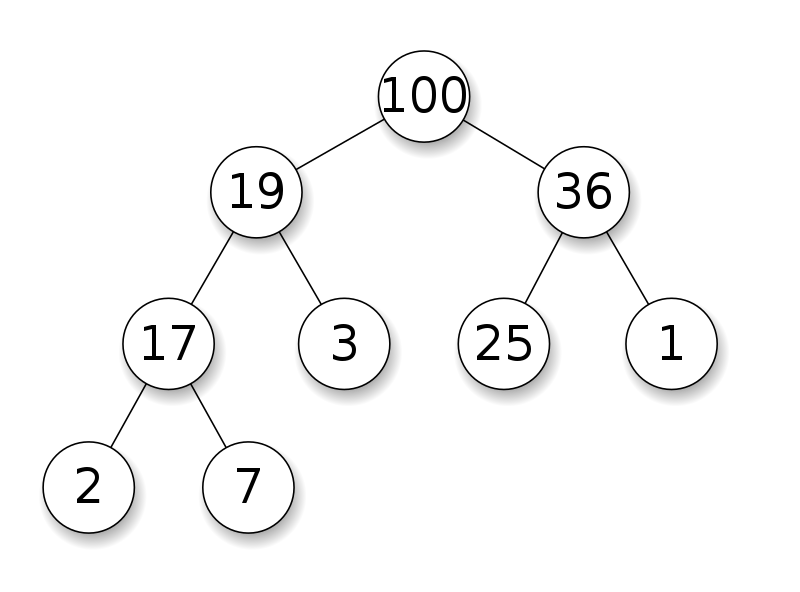
\includegraphics{Max-Heap.png}
\end{center}
\begin{center}
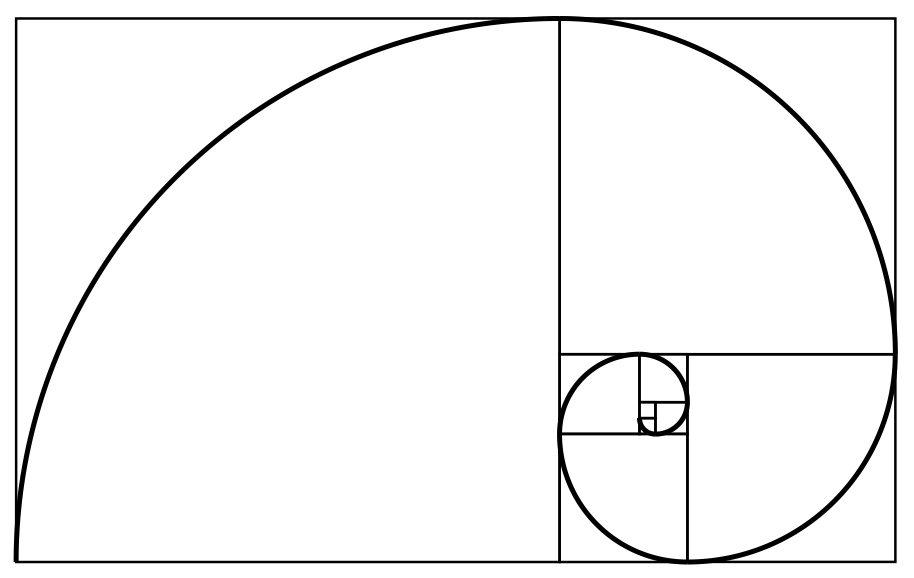
\includegraphics{fibonacci.svg}
\end{center}


\newpage
%\nocite{*}
%\printbibliography

\end{document}

